346. На квадратном поле $4\times4$ клетки растут цветы, число цветов в каждой клетке указано на схеме. Вася начинает с левой нижней клетки (с числом 2) и, переходя каждый раз в соседнюю справа или сверху, добирается до правой верхней клетки, собирая цветы с клеток, на которых побывал. Сколько есть маршрутов, на которых Вася соберёт ровно 43 цветка?\\
\begin{figure}[ht!]
\center{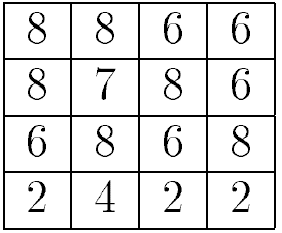
\includegraphics[scale=0.35]{flow2.png}}
\end{figure}\\
